% !TEX root = ../BScWIMEngl.tex

\chapter{Reinforcement Learning Algorithms}

\section{Introduction}

Dynamic Programming usually breaks down in the real world for two reasons:
\begin{enumerate}
    \item The transition probabilities and immediate rewards are not known or hard to calculate.
    \item The state and action space is too large to even compute one iteration of Dynamic Programming for every state-action tuple (e.g. possible positions and possible moves in every position in chess).
\end{enumerate}

This is where \emph{Reinforcement Learning} algorithms come in, which try to find solutions without having to sweep the entire state space. In this chapter based on \textcite{suttonReinforcementLearningIntroduction2018a} we will examine advantages and disadvantages of various algorithms and discuss possible variations and extensions. In the next chapter we will show almost sure convergence of the basic algorithms introduced in this chapter and illustrate their connection to sotchastic approximation. \fxwarning{check outline of the plan} 

We separate their introduction and the convergence proofs, because -- while the guarantee of almost sure convergence is reassuring -- it is of little use for comparing various algorithms. Since one of the reasons for moving away from Dynamic Programming in the first place was, that we could not calculate the value function for the entire state space within a reasonable time frame. As the size of the state space is often too large for that.  Therefore almost sure convergence should not be viewed as more than an entry requirement. For this reason most papers compare algorithms empirically on various example problems. And for some of the more complex algorithms convergence proofs simply do not exist yet. 

So since the theoretical convergence properties are usually only ever an afterthought, it is more natural to introduce the various algorithms heuristically, explaining what specific problems they try to address with examples.


But let us ignore the second problem for a moment and consider the case where we only have the first problem (\(p\) and \(r\) unknown). Then we can learn from a sample \(((X_t, A_t, Y_t, R_t), t\in\{0,\dots, T\})\) with
\[
	(Y_t,R_t)\sim \cP(\cdot \mid X_t, A_t)
\]
and with \(Y_t=X_{t+1}\) if the sample is generated sequentially by a behavior. But there is no reason not to allow this more general sample which might be useful in cases where you can jump around in the statespace and try different transitions at will. 

We can then use this batch of transitions to calculate estimators \(\hat{p},\hat{r}\) for the state transitions and immediate rewards \(\hat{r}\). And use Dynamic Programming on these estimators.

%Since the transition probabilities and immediate rewards are not known, these algorithms first need to create samples from which to estimate them. These samples are created using a behavior resulting in a state-action-reward sequence \((X_t,A_t,R_t,t\in\N_0)\). This behavior has to explore the state-action space, trying to generate data of interesting transitions. From this the algorithm then has to estimate the value functions. 


\begin{algorithm}
	\caption{Naive Batch Learning Algorithm} \label{naive batch learning algorithm}
	\begin{enumerate}
		\item Generate the history \((X_t, A_t, Y_t, R_t, t\in\{0,\dots, T\})\)
		\begin{algorithmic}[1] 
			\For{ \((y,x,a)\in\cX\times\cX\times\cA \)} \Comment{initialize variables}
				\State rewards[\(x,a\)]\(\gets\)list() 
				\State stateTransitions[\(y\mid x,a\)]\(\gets\) 0
				\State totalTransitions[\(x,a\)]\(\gets\) 0
			\EndFor
			\For{\(t=0,\dots, T\)}
				\State rewards[\(X_t,A_t\)].append(\(R_{t+1}\))
				\State stateTransitions[\(Y_t\mid X_t,A_t\)]\(++\) \label{algo1: incr 1}
				\State totalTransitions[\(X_t,A_t\)]\(++\)\label{algo1: incr 2}
			\EndFor
			\For{\((x,a)\in\cX\times\cA\)}
				\State \(\hat{r}(x,a) \gets\) average(rewards[x,a])
				\For{\(y\in\cX\)}
					\State \(\hat{p}(y\mid x,a)\gets\) stateTransitions[\(y\mid x,a\)]\(/\)totalTransitions[\(x,a\)]\label{calculation of hat p}
				\EndFor
			\EndFor
		\end{algorithmic}
		\item Use Dynamic Programming on \(\hat{r}\), \(\hat{p}\) 
	\end{enumerate}
\end{algorithm}
\fxnote{add code/ ref code Dynamic Programming}
\fxnote{numerical stability analysis?}

If the batch was generated by an exploration policy we separated the \emph{exploration} from the later \emph{exploitation}. The methods which do that are often grouped under the term \emph{Batch Reinforcement Learning} or \emph{off-line} learning. 

This method works fine, if the state space is small and one can sample enough observations for every state and action in a reasonable timeframe.
But if our state space is too large for that, it is impractical to wait for this. 

%%%%%%%%%%%%%%%%%%%
\section{Monte Carlo}
%%%%%%%%%%%%%%%%%

One idea to tackle larger state spaces is, that it is often unneccessary to know the value function in every state.

To visualize this idea it is useful to imagine the state space to be a room the agent has to navigate. 

\[
\begin{tikzpicture}
	\foreach \x in {0,1,2,3,4}{
		\foreach \y in {0,1,2,3,4}{
			\draw (\x,\y) rectangle +(1,1);
		}
	}
	\node at (1.5,0.5){S};
	\node at (2.5,4.5) {\textcolor{gray}{\(\gamma\)}};
	\foreach \value in {2,3,4,5}{
		\tikzmath{
			int \power;
			\power=7-\value;
		}
		\node at (1.5, \value-0.5) {\textcolor{gray}{\(\gamma^\power\)}};
	}
	\node at (3.5, 4.5){G};
	

	\node at (8.5,2.5) {\parbox[t]{6cm}{The state space \(\cX\) are the tiles on the floor, the actions \(\cA\) are the adjacent tiles, where the next state is with probability one equal to the action, and the reward is 0 for every transition but the transition to the goal (G) where the reward is 1 and the game ends. The start state is S. The value of choosing a tile is indicated in grey on the tile.}};
\end{tikzpicture}
\]

It is often enough for the agent to know the action value function for the states on his path, without knowing the value of states in the corners. Since he can then follow these ``breadcrumbs'' to find the goal reliably again. And it will quickly stop walking in circles if it goes into the direction of the highest value next time. 

This idea is the basis for Monte Carlo algorithms. To make notation more brief we will introduce the algorithm to calculate the value function, the action value function will be analogous. Consider an episodic MDP and a behavior \(\pi\) then
\[
	\sum_{t=0}^\infty\gamma^tR_{t+1}=\sum_{t=0}^T\gamma^tR_{t+1}
\]
is a bias free estimator for \(V^\pi(X_0)\) for episode lenght T. As the definition was
\[
	V^\pi(x)=\E\left[\sum_{t=0}^\infty\gamma^tR_{t+1} \;\middle|\; X_0=x \right] 
\]
And because of the markov property
\[
	\sum_{t=k}^T\gamma^tR_{t+1}
\]
is a bias free estimator for \(V^\pi(X_k)\). \emph{First-visit Monte Carlo} uses the return after the first visit of a state \(x\in\{X_1,\dots,X_t\}\) as an estimator for \(V^\pi(x)\).

\begin{algorithm}
	\caption{First-visit Monte Carlo}
	\begin{algorithmic}[1]
		\For{\(x\in\cX\)} \Comment{initializing}
			\State Returns\((x)\gets\) list()
			\State \(V^\pi(x)\gets 0\)
		\EndFor
		\While{true} (forever) \Comment{learning}
			\State Generate an episode \(((X_t,R_{t+1}), t\in\{0,\dots,T\})\) with behavior \(\pi\)
			\For{\(x\in\{X_0,\dots,X_T\}\)}
				\State \(k\gets \min\{t \mid X_t=x\}\)
				\State Returns\((x)\).append(\(\sum_{t=k}^T\gamma^tR_{t+1}\))
				\State \(V^\pi(x)\gets\) average(Returns(x))
			\EndFor
		\EndWhile
	\end{algorithmic}
\end{algorithm}

Because of the strong law of large numbers, first-visit Monte Carlo algorithm causes the value function estimation \(\hat{V}^\pi(x)\) to converge with probability 1 to \(V^\pi(x)\) for every state \(x\in\cX\) which is visited with positive probability given behavior \(\pi\) and starting distribution \(X_0\). 

\emph{Every-visit} Monte Carlo uses the Return after every visit of a state \(x\) to estimate \(V^\pi(x)\). Since this means that the tail of the rewards can be included in multiple returns, the returns are not independent from each other anymore which make proving convergence a little bit more difficult than simply applying the strong law of large numbers. But every visit Monte Carlo will turn out to be a special case of \(TD(\lambda)\).\fxnote{will TD proof work?} 

The same method can be applied to learn the action value function \(Q^\pi\). In this case we take the returns following a state \emph{and} action as estimators for \(Q^\pi\). But if the model is known and our problem is just a large state space calculating \(V^\pi\) is preferrable, since \(|\cX|\le |\cX\times\cA|\) means that the first algorithm needs fewer observations to converge and \(Q^\pi\) can be calculated with \(V^\pi\) given \(r\) and \(p\).

\subsection{From \(\pi\) to \(\pi^*\)}
Let us assume exploring starts 
\[
	\Pr(X_0=x)>0 \qquad \forall x\in\cX
\] 
for a moment. Then Monte Carlo converges whatever policy we select. Similar to policy iteration (\ref{policy iteration}) we can then alternate between calculating \(Q^{\pi_n}\) and selecting \(\pi_{n+1}\) as a greedy policy with regard to \(Q^{\pi_n}\). This is referred to as generalized policy iteration (GPI). If we would wait for our Monte Carlo approximation of \(Q^{\pi_n}\) to converge, \(\pi_n\) would converge to \(\pi^*\) for the same reason as policy iteration converges. But remember we are doing Monte Carlo in the first place, because the state space is too large to wait for an evaluation of every state. Which means in practice algorithms alternate beteen choosing a greedy policy with regard to \({V^{\pi_n}}\) and generating an episode with policy \(\pi_n\), averaging the estimates from this episode with the estimates of \(V^{\pi_{n-1}}\). But since we have to assume
\[
	V^{\pi_{n-1}}\neq V^{\pi_n}
\] 
in general, using these old estimates is not bias free. It is easy to see that this procedure can only converge to \(\pi^*\) if it converges at all. Since there are only a finite number of deterministic stationary policies it would have to stay constant at some point, but for a constant policy Monte Carlo will converge, and then the policy can only stay constant if it is greedy with regards to its own value function, which forces it to be optimal (\ref{real improvement or optimal}). But it is still an open problem whether or not this alternating procedure converges at all \parencite[99]{suttonReinforcementLearningIntroduction2018a}.

If we remove the assumption of exporing starts, we still need to ensure that every state is visited with positive probability for MC to converge. This requires the policy to do the exploring. There are multiple approaches to exploration \fxnote*{check claim}{which we will discuss later}. We will discuss the most straightforward example here, under the assumption that we can calculate \(Q^{\pi_n}\) somehow.  

\begin{definition}
	A stationary policy \(\pi\) is called 
	\begin{description}[font=\normalfont]
		\item[\emph{soft}] if it fulfills 
		\[
			\pi(a\mid x)>0 \qquad\;\; \forall (x,a)\in\cX\times\cA
		\]
		\item[\emph{\(\vep\)-soft}] if it fulfills 
		\[
			\pi(a\mid x)>\frac{\vep}{|\cA_x|} \quad \forall (x,a)\in\cX\times\cA
		\]
		\item[\emph{\(\vep\)-greedy}] with regard to Q, if it selects the greedy action w.r.t. Q with probability \((1-\vep)\) and a (uniform) random action with probability \(\vep\), i.e. \[\pi(a\mid x)=
			\begin{cases}
				(1-\vep)+ \frac{\vep}{|\cA_x|} & a \text{ is greedy\footnotemark[1]}\\
				\frac{\vep}{|\cA_x|} & a \text{ is not greedy}
			\end{cases}
		\]
	\end{description}\footnotetext[1]{w.l.o.g. only one greedy action}
	Note that an \(\vep\)-greedy policy is \(\vep\)-soft.

	An \(\vep\)-soft policy \(\pi^*\) is called \emph{\(\vep\)-soft optimal} if 
	\[
		V^{\pi^*}(x)=\sup_{\pi\; \vep\text{-soft}}(x) V^\pi \eqqcolon \tilde{V}^*(x)
	\]
\end{definition}

\begin{prop}
	Generalized policy iteration with \(\vep\)-greedy policies converges to a \(\vep\)-soft optimal policy
\end{prop}
\begin{proof}
	% Let \(\pi_{n+1}\) be \(\vep\)-greedy with regard to \(Q^{\pi_n}\). Since \(\pi_n\) is an \(\vep\)-soft policy we know that
	% \[
	% 	\pi_n(a\mid x) -\frac{\vep}{|\cA_x|} \ge 0
	% \]
	% which together with the equality
	% \[
	% 	\sum_{a\in\cA_x}\frac{\pi_n(a\mid x) -\frac{\vep}{|\cA_x|}}{1-\vep} 
	% 	= \frac{\left(\sum_{a\in\cA_x}\pi_n(a\mid x)\right)- \vep}{1-\vep}
	% 	= 1
	% \]
	% implies the inequality (\ref{weighted sum}). Since the maximum is larger than the weighted average.
	% \begin{align}
	% 	&T^{\pi_{n+1}}V^{\pi_n}(x)=Q^{\pi_n}(x,\pi_{n+1}(x))
	% 	=\sum_{a\in\cA_x} \pi_{n+1}(a\mid x) Q^{\pi_n}(x,a)
	% 	\nonumber\\
	% 	&\lxeq{\vep\text{-greedy}}\frac{\vep}{|\cA_x|}\sum_{a\in\cA_x}Q^{\pi_n}(x,a)
	% 	+(1-\vep)\max_{a\in\cA_x} Q^{\pi_n}(x,a)
	% 	\nonumber\\
	% 	&\ge\frac{\vep}{|\cA_x|}\sum_{a\in\cA_x}Q^{\pi_n}(x,a) 
	% 	+(1-\vep)\sum_{a\in\cA_x}
	% 	\frac{\pi_n(a\mid x) -\frac{\vep}{|\cA_x|}}{1-\vep}Q^{\pi_n}(x,a)  
	% 	\label{weighted sum}\\
	% 	&=\frac{\vep}{|\cA_x|}\sum_{a\in\cA_x}Q^{\pi_n}(x,a) 
	% 	-\frac{\vep}{|\cA_x|}\sum_{a\in\cA_x}Q^{\pi_n}(x,a)
	% 	+\sum_{a\in\cA_x}\pi_n(a\mid x)Q^{\pi_n}(x,a)
	% 	\nonumber\\
	% 	&=V^{\pi_n}(x)\nonumber
	% \end{align}
	% This implies \(V^{\pi_{n+1}}\ge V^{\pi_n} \). 
	To use the same argument as with the standard policy iteration, we would need
	\[
		T^*(V^{\pi_n})=T^{\pi_{n+1}}(V^{\pi_n})
	\]
	But this is not true. To circumvent this problem we ``move the requirement of \(\vep\)-softness into the environment''. I.e. we define an MDP \(\tilde{M}\) where
	\[
		\tilde{\cP}(\cdot \mid x,a) \coloneqq (1-\vep) \cP(\cdot \mid x,a) 
		+ \frac{\vep}{|\cA_x|}\sum_{b\in\cA_x} \cP(\cdot \mid x,b)
	\]
	This means, that with probability \(\vep\) the transition kernel will ignore the selected action and behave as if an uniformly random action was chosen.	
	
	We can transform \(\vep\)-soft policies \(\pi\) from the old MDP to stationary policies \(\tilde{\pi}\) of \(\tilde{M}\) with a mapping \(f\), where
	\[
		f(\pi)(a\mid x)=\tilde{\pi}(a\mid x)\coloneqq \frac{\pi(a\mid x)-\frac{\vep}{|\cA_x|}}{1-\vep}\ge 0
	\]
	And for every stationary policy \(\tilde{\pi}\) of \(\tilde{M}\) we can define the \(\vep\)-soft policy \(\pi\) by
	\[
		\pi(a\mid x)\coloneqq (1-\vep)\tilde{\pi}(a\mid x) + \frac{\vep}{|\cA_x|}
	\]
	which is the inverse mapping. Therefore \(f\) is a bijection between the \(\vep\)-soft policies in the old MDP and all stationary policies in the new MDP. We now show that the Value functions \(V^\pi\) stay invariant with regard to this mapping. 
	First note that
	\begin{align*}
		\tilde{p}(y\mid x,a)
		&=\tilde{\cP}(\{y\}\times \R\mid x,a)\\
		&=(1-\vep)p(y\mid x,a)+\frac{\vep}{|\cA_x|}\sum_{b\in\cA_x}p(y\mid x,b)
	\end{align*}
	and together with \(q(B\mid x,a)\coloneqq \cP(\cX\times B \mid x,a)\) the complementary marginal distribution we can show
	\begin{align*}
		\tilde{r}(x,a)&=\int t\ d\tilde{q}(t \mid x,a)=\int t\ 
		d\left((1-\vep)q(\cdot\mid x,a) + \frac{\vep}{|\cA_x|}\sum_{b\in\cA_x}q(\cdot\mid x,b)\right)(t) \\
		&=(1-\vep)\int t\ dq(t\mid x,a) 
		+ \frac{\vep}{|\cA_x|}\sum_{b\in\cA_x} \int t\ dq(t\mid x,a)\\
		&=(1-\vep)r(x,a) + \frac{\vep}{|\cA_x|}\sum_{b\in\cA_x}r(x,b)
	\end{align*}
	Therefore we know
	\begin{align*}
		&\sum_{a\in\cA_x}\tilde{\pi}(a\mid x)\tilde{r}(x,a)\\
		&=\sum_{a\in\cA_x} \left(\frac{\pi(a\mid x)-\frac{\vep}{|\cA_x|}}{1-\vep} \right)
		\left((1-\vep)r(x,a) + \frac{\vep}{|\cA_x|}\sum_{b\in\cA_x}r(x,b)\right)\\
		&=\sum_{a\in\cA_x}\left(\pi(a\mid x)-\frac{\vep}{|\cA_x|}\right)r(x,a) 
		+ \frac{\vep}{|\cA_x|}\sum_{b\in\cA_x}r(x,b) 
		\underbracket[1pt]{\sum_{a\in\cA_x}\frac{\pi(a\mid x)-\frac{\vep}{|\cA_x|}}{1-\vep}}_{
			=1
		}\\
		&=\sum_{a\in\cA_x}\pi(a\mid x)r(x,a)
	\end{align*}
	and similarly
	\begin{align*}
		&\Pr^{\tilde{\pi}}(\tilde{X}_1=y\mid \tilde{X}_0=x) 
		=\sum_{a\in\cA_x}\tilde{\pi}(a\mid x)\tilde{p}(y\mid x,a)\\
		&=\sum_{a\in\cA_x}\left(\frac{\pi(a\mid x)-\frac{\vep}{|\cA_x|}}{1-\vep} \right)
		\left((1-\vep)p(y\mid x,a)+\frac{\vep}{|\cA_x|}\sum_{b\in\cA_x}p(y\mid x,b)\right)\\
		&=\dotsc = \sum_{a\in\cA_x} \pi(a\mid x)p(y\mid x,a) =\Pr^\pi(X_1=y\mid X_0=x)
	\end{align*}
	The last two equations together imply
	\begin{align*}
		\tilde{T}^{\tilde{\pi}}V^\pi(x)&=\sum_{a\in\cA_x}\tilde{\pi}(a\mid x)\tilde{r}(x,a) 
		+ \gamma \sum_{y\in\cX}\Pr^{\tilde{\pi}}(\tilde{X}_1=y\mid X_0=x)V^\pi(y)\\
		&=\sum_{a\in\cA_x}\pi(a\mid x)r(x,a) + \gamma \sum_{y\in\cX}\Pr^\pi(X_1=y\mid X_0=x)V^\pi(y)\\
		&=T^\pi V^\pi(x)=V^\pi(x)
	\end{align*}
	Since the fixpoint is unique it follows that
	\[
		V^{\tilde{\pi}}=V^\pi
	\]
	Since f is bijective this implies
	\[
		\sup_{\tilde{\pi}\in \tilde{\Pi}_S}V^{\tilde{\pi}}(x)=\sup_{\pi\ \vep\text{-soft}} V^\pi(x)
	\]
	as well as
	\begin{align*}
		Q^{\tilde{\pi}}(x,a)&=\tilde{r}(x,a)+\gamma \sum_{y\in\cX} \tilde{p}(y\mid x,a) V^\pi(y)\\
		&=\begin{aligned}[t]
			&(1-\vep)\left(r(x,a)+\gamma \sum_{y\in\cX}p(y\mid x,a) V^\pi(y) \right)\\
			&\qquad + \frac{\vep}{|\cA_x|}\sum_{b\in\cA_x}\left(r(x,b)+\gamma \sum_{y\in\cX}p(y\mid x,b) \right)
		\end{aligned}\\
		&=(1-\vep)Q^\pi(x,a)
		+ \frac{\vep}{|\cA_x|}\sum_{b\in\cA_x}\left(r(x,b)+\gamma \sum_{y\in\cX}p(y\mid x,b) \right)
	\end{align*}
	Which implies that
	\[
		\arg\max_{a\in\cA_x} Q^{\tilde{\pi}}(x,a)=\arg\max_{a\in\cA_x} Q^\pi(x,a)
	\]
	Threfore greedy with regard to \(Q^\pi\) and \(Q^{\tilde{\pi}}\) is the same. Let \(\pi_n\) be an \(\vep\)-soft policy, and let \(\pi_{n+1}\) be \(\vep\)-greedy with regard to 
	\(Q^{\pi_n}\). Then \(\tilde{\pi}_{n+1}\coloneqq f(\pi_{n+1})\) is greedy w.r.t. 
	\(Q^{\tilde{\pi}_n}\)
	\begin{align*}
		\tilde{\pi}_{n+1}(a\mid x)&=f(\pi_{n+1})(a\mid x)
		=\frac{\pi(a\mid x)-\frac{\vep}{|\cA_x|}}{1-\vep}\\
		&=\begin{cases}
			\frac{\left((1-\vep) + \frac{\vep}{|\cA_x|}\right) -\frac{\vep}{|\cA_x|}}{1-\vep}=1 & a \text{ is greedy}\\
			\frac{\frac{\vep}{|\cA_x|}- \frac{\vep}{|\cA_x|}}{1-\vep}=0 & a \text{ is not greedy}
		\end{cases}
	\end{align*}
	This finishes our proof
	\[
		\sup_{\pi\ \vep\text{-soft}} V^\pi(x)
		=\sup_{\tilde{\pi}\in \tilde{\Pi}_S}V^{\tilde{\pi}}(x)
		=\lim_{n\to\infty} V^{\tilde{\pi}_n}(x)
		=\lim_{n\to\infty} V^{\pi_n}(x)
		\qedhere
	\]
\end{proof}


\subsection{Shortcomings of Monte Carlo}
\citeauthor{suttonReinforcementLearningIntroduction2018a} provides a very instructive example for the weakness of Monte Carlo. Recall that Monte Carlo tries to estimate \(V^\pi\). So the example assumes a given behavior and tries to evaluate the value of a situation.

\begin{example}[Driving Home]
	Let us assume that John Doe works in city A and drives to his home in city B after work every day. Since he wants to get home as quickly as possible, the value of the state is antiproportional to the time it will take him from a certain position home. This means that estimating the value of a certain state is equivalent to estimating the time left to drive. The longer John drives this route the better he will get at estimating the time it will take him to drive certain sections of the road. If there is a delay in an earlier section he has a good estimate for the remaining time once he cleared the obstruction. Now imagine he is driving home from a doctors appointment from city A. As soon as he enters the highway to city B, he is able to use his experience driving this route to estime the remaining time quite precisely.

	The Monte Carlo algorithm on the other hand \emph{never} uses existing value estimations to estimate the value of a different state. If John Doe uses Monte Carlo estimates to guess the remaining time from the doctor, the accuracy of his estimates will only ever increase with the times he actually starts driving from the doctor's office. 
\end{example}

Since Monte Carlo has more possible "starting points" or generally earlier points in the chain in case of estimating \(Q^\pi\), it is worse in this case. An extreme example would be two actions in the same state which have the same effect. Even though Monte Carlo might have a good estimate of the value of the first action it will start completely anew for the second action. 
\fxnote{illustrations?}

\section{Temporal Difference Learning TD}
Temporal Difference learning (TD) first proposed by \textcite{suttonLearningPredictMethods1988} addresses this weakness of Monte Carlo algorithms. For a sequence \((X_t,A_t,R_{t+1},t\in\N_0)\) realized\fxnote{realized?} with a stationary behavior \(\pi\), we know that
\begin{align}
	&\E^\pi[R_{t+1}+\gamma V(X_{t+1})\mid X_t=x] 
	\nonumber\\
	&=\E^\pi[r(x,A_0)\mid X_0=x]+\gamma\sum_{y\in\cX}\Pr^\pi(X_1=y\mid X_0=x)V(y) 
	\nonumber\\
	&= T^\pi V(x) \label{estimates T^pi V}
\end{align}
The random variable \(R_{t+1}+\gamma V(X_{t+1})\) is therefore a bias free estimator for \(T^\pi V (X_t)\). But because of its variance we can not simply update \(V(X_t)\). Instead TD moves the estimate into the direction of this observation. To get an intuition for why this makes sense consider this example.
\begin{example}[Unwinding the Arithmetic Mean]\label{unwinding the mean}
	\begin{align*}
		\widebar{X}_n&=\mfrac{1}{n}\sum_{i=1}^n X_i 
		= \mfrac{n-1}{n}\mfrac{1}{n-1}\sum_{i=1}^{n-1}X_i +\mfrac{1}{n}X_n\\
		&=\left(1-\mfrac{1}{n}\right)\widebar{X}_{n-1}+\mfrac{1}{n}X_n \\
		&= \widebar{X}_{n-1} + \underbracket[1pt][1.3ex]{\frac{1}{n}}_{\text{\clap{``learning rate''}}}\underbracket[1pt][0.4ex]{(X_n - \widebar{X}_{n-1})}_{\text{``direction''}}
	\end{align*}
\end{example}

But Temporal Difference Learning tries to do Dynamic Programming (i.e. replacing \(V\) with \(T^\pi V\), which would require a learning rate of \(1\)) at the same time as trying to reduce the error of the estimate of \(T^\pi V\), where the learning rate should be something like \(1/n\). The smaller the learning rate, the more of the old estimate we retain. This has the disadvantage that old estimates are (in a way) previous steps in dynamic programming, which are further away from \(V^\pi\). Larger learning rates on the other hand retain more of the variance of the latest random variable in the estimator. So one might for example want to have larger steps at the beginning until the dynamic programming part converges and then start to focus more on the variance reduction part. This implies that a wider range of learning rates might be sensible. We therefore define 
\begin{align}\label{TD learning}
	V_{n+1}(x) \coloneqq
	\begin{cases}
		V_n(x)+\alpha_n(x)[R_{n+1}+\gamma V_n(X_{n+1}) - V_n(x)] & x=X_n\\
		V_n(x) & x\neq X_n
	\end{cases}
\end{align}
where \(\alpha_n\) is called the \emph{learning rate}. As one might want to increase the learning rates for rarely visited areas of the MDP, and decrease it for well known parts, it makes sense to allow it to be a function of the history \(((X_t, A_t, R_{t+1}), t\in\{0,\dots, n\})\) and thus allow it to be a random variable. We will omit this possible dependency for now and reconsider it in chapter \ref{stoch apprx}.

For a deterministic stationary behavior \(\pi\), we can show the analogue 
\begin{align*}
	&\E^\pi[R_{t+1}+\gamma Q(X_{t+1}, A_{t+1})\mid X_t=x, A_t=a]\\
	&=r(x,a) +\gamma \sum_{y\in\cX}p(y\mid x,a)Q(y,\pi(y))\\
	&= T^\pi(Q)(x,a)
\end{align*}
\fxnote{Do I need to generalize the def?}
Note that we could easily extend this to all stationary policies (c.f. \ref{expand Q^pi}, \ref{T^pi unique}), by defining
\[
	T^\pi Q(x,a)\coloneqq r(x,a) +\gamma \smashoperator{\sum_{(y,b)\in\cX\times\cA}}\Pr^\pi[X_{t+1}=y,A_{t+1}=b\mid X_t=x,A_t=a]Q(y,b)
\]

Similar to the Monte Carlo algorithm we use generalized policy iteration to approach \(\pi^*\). But since we do not need to wait for an espisode to finish to create new estimates, we can alternate even more quickly between calculating \(Q^{\pi_n}\) and selecting \(\pi_{n+1}\). The most extreme form is now updating the policy before every transition in every time step. This is what is called \emph{on-line} learning in contrast to the \emph{off-line} mentioned in the introduction. 

Batch Reinforcement Learning is often used synonymously with off-line learning. But as batch learning algorithms were designed to utilize the information of the existing batch as efficiently as possible, there were some attempts to modify them in order to provide intermediate results to advise action selection, transforming them into on-line algorithms. \textcite{langeBatchReinforcementLearning2012} suggest to refer to these algorithms as \emph{growing batch reinforcement learning}. We will discuss an example in \ref{growing batch learning} after explaining the the need for it. 

\begin{algorithm}
	\caption{On-line TD GPI \parencite{suttonReinforcementLearningIntroduction2018a}}
	Assume there is a mapping \(\Psi\) assigning an action value function Q a policy \(\pi\) (for example mapping Q on an \(\vep\)-greedy policy w.r.t. Q).
	\begin{algorithmic}[1]
		\State initialize Q(x,a)
		\While{True} \Comment{for each episode}
			\State initialize \(x\) \Comment{Start state}
			\State choose \(a\) according to \(\Psi(Q)(\cdot \mid x)\)
			\Repeat \Comment{for each step of an episode}
				\State do \(a\), observe reward \(R\) and next state \(y\)
				\State choose \(b\) according to \(\Psi(Q)(\cdot \mid y)\)
				\State \(Q(x,a)\gets Q(x,a) + \alpha_n(x,a) [R+\gamma Q(y,b) -Q(x,a) ]\)
				\State \(x\gets y\); \(a\gets b \); \Comment{next state and action are current}
			\Until{x is terminal}
		\EndWhile
	\end{algorithmic}
	Where \(\alpha_n\) is the learning rate.
\end{algorithm}

\subsection{Shortcomings of TD} \label{shortcomings TD}
In a way TD is the opposite of Monte Carlo. While Monte Carlo did not use existing estimates of the value function, TD \emph{only} uses existing estimates. This can cause problems as well.


\begin{wrapfigure}{r}{6cm}
	\begin{center}
		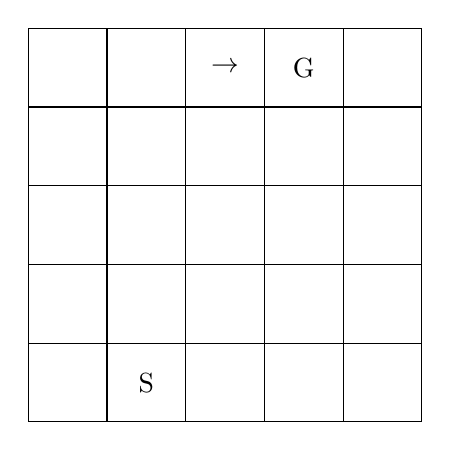
\begin{tikzpicture}
			\foreach \x in {0,1,2,3,4}{
				\foreach \y in {0,1,2,3,4}{
					\draw (\x,\y) rectangle +(1,1);
				}
			}
			\node at (2.5,4.5){\(\rightarrow\)};
			\node at (1.5,0.5){S};
			\node at (3.5, 4.5){G};
		\end{tikzpicture}
	\end{center}
\end{wrapfigure}

 Recall our room navigation example and assume that we initialize the TD algorithm with the value function \({Q\equiv 0}\). Then the algorithm picks an action, walks into that direction, gets reward zero and updates \(Q\) in this place to zero. This continues until it reaches the goal where it updates the state and action that led it to the goal with a positive number. This makes this action the greedy action, which we indicate with an arrow. But in all the previous states TD still does not behave better than before. It will take a couple more episodes to backpropagate the reward of the goal to the \(Q\) values at the start. This is quite bad in comparison to Monte Carlo which only takes one episode to leave a trail of breadcrumbs to the goal. One way to tackle this problem is to try to find a compromise between Monte Carlo and TD which \(TD(\lambda)\) tries to do. The other approach is growing batch learning. 


\subsection{Growing Batch Learning}\label{growing batch learning} \fxnote{section instead of subsection? chance place? - after TD(lambda), after Q-learning?}
One reason for TD's problems is, that it uses sampled transitions only once and then throws them away. This is not so much a problem when the MDP is cheap to sample. But in a lot of real world applications experiences cost more time than most computations, can be expensive (causing damage to hardware) and/or outright dangerous (e.g. self-driving cars). For this reason it is preferrable if the algorithm learns as much as possible from a given batch of experiences (transitions). To serve as a comparison, recall our initial naive batch learning algorithm (Algorithm \ref{naive batch learning algorithm}). First it estimates the model parameters; after that it uses these estimates multiple times in every Dynamic Programming step. TD's estimates, on the other hand, are baked into the current estimate of \(V\) (or \(Q\)), which means that older samples are baked into older instances of \(V\) which can not really be reused as they also represent previous instances of the ``dynamic programming part'' of TD (and maybe also previous policies in the GPI case with \(Q\)).

So how could we modify this batch learning algorithm (using the entire batch of transitions) to be on-line, i.e. provide provisonal estimates and incorporate additional information -- growing batches?

First we can notice that we estimate \(\hat{r}\) by calculating the algorithmic mean, which we can unwind as in \ref{unwinding the mean}. But note that this increases the number of operations for calculating the mean of \(n\) elements from 
\[
	n-1 \text{ additions } + 1\text{ division} = n
\]
to 
\[
	(n-1) \times (1\text{ addition} + 1 \text{ subtraction } + 1\text{ division})=3n - 3 
\]
basically tripling the number of operations. 

The calculation of \(\hat{p}\) is already partly on-line, as the increment  in line \ref{algo1: incr 1} and \ref{algo1: incr 2} can be done in every transition. Recalculation of  \(\hat{p}\) in every step would entail an iteration through all the \(y\in\cX\) whichever followed a particular \((x,a)\) and might thus be better left for the time that \(\hat{p}\) is actually required.

To accelerate Dynamic Programming we could use the previous estimation of \(V\) (\(Q\)) as a starting point the next time we use DP. But DP still requires us to go over the entire state space (state-action space) for just one update, and most model parameter stay the same anyway so more local updates are warranted.

The approach of algorithms like ``Dyna'' are basically hybrids of a ``pure'' on-line learning algorithm like TD (or -- as we will later see -- Q learning i.e. Dyna-Q) and a model based learning algorithm which runs in the background -- ideally (for performance) as a separate process -- and updates the value function with ``localized'' dynamic programming, i.e.
\begin{align}
	\label{async DP V}
	V^\pi(x) \gets \sum_{a\in\cX_x}\pi(a\mid x) \left( \hat{r}(x,a) + \sum_{y\in\cX} \hat{p}(y\mid x,a) V^\pi(y)\right)
\end{align}
or
\begin{align}\label{async DP Q}
	Q^\pi(x,a) \gets \hat{r}(x,a) + \sum_{y\in\cX}\sum_{b\in\cA_y} \hat{p}(y\mid x,a) \pi(b\mid y) Q^\pi(y,b)
\end{align}
This leaves us with the question, which states to prioritize for updates. The simplest form of Dyna just picks these states randomly. From our example in \ref{shortcomings TD} it should be quite obvious, that this is not the most efficient way to backpropagate rewards. But it should not be completely disregarded as it has one of, if not \emph{the} smallest overhead of possible selection algorithms. 

A second approach is \emph{prioritized sweeping} where the absolute difference between the sample of \(T^\pi V(X_t)\), \(R_{t+1}+\gamma V(X_{t+1})\) and \(V(X_t)\) (c.f. (\ref{TD learning})) needs to be larger than a certain threshold for this state to be put into the update queue. The model learning part then updates all the states which lead to this state, and inserts theses states into the queue themselves if their change is large too. \fxnote{write down algorithm?}

Another approach is \emph{trajectory sampling} where a trajectory of state is generated by applying the current policy to the model (\(\hat{p}\)) of the real MDP. Then the alogrithm could update the value functions along this chain of states, ideally backwards (to avoid the problem that TD has). This focuses the update on parts of the MDP which are actually relevant as they are possible to reach with the current policy. Just like it makes more sense to analyse different chess games as a joint string of moves instead of analysing random positions which might never come up in a real game. Trajectory sampling can also be combined with the other approach to improve TD. By using the learning algorithm of the mixture \(TD(\lambda)\) of TD and Monte Carlo on these simulated trajectories. 

The approaches we discussed here so far are all \emph{model based learning}, which could leave the impression that (growing) batch learning is synonymous with model based learning in contrast to \emph{model free learning} methods like Monte Carlo and TD, which do not actually estimate the transition probabilities and skip right to the value functions. But there are also model free growing batch learning methods. 

One such example is \emph{experience replay} coined by \textcite{linSelfimprovingReactiveAgents1992} which simply creates backups of past transitions and plays them back to the learning algorithms in a possibly different (e.g. backwards) order. The fact, that playing back a random transition is equivalent to sampling the model (\(\hat{p}, \hat{r}\)), motivates why this has the desired effect if the selection of past transition is not unbalanced.  Experience replay can be warranted if the sums in (\ref{async DP V}) or (\ref{async DP Q}) are too large, i.e. when too many different states \(y\) can follow a state \(x\). This is sometimes described as a high \emph{branching factor}, where this factor could be defined as the average number of branches. Experience replay esentially trades memory (backing up all transitions) for computation speed, as it does not need to sum over all branches following a state.

\textcite{suttonReinforcementLearningIntroduction2018a} call the model based learning methods ``planning'', and use the term ``decision time planning'' for algorithms which try to improve the knowledge of \(Q(X_t,a)\) for all actions \(a\), just before selecting the action \(A_t\), by exploring the branches of the state based on its current model (essentially applying some localized Dynamic Programming to its model to aid the decision).



\section{TD(\(\lambda\)) --  Mixing Monte Carlo and TD} 
To try and mix TD and Monte Carlo, recall that Monte Carlo uses 
\[
	\hat{V}^\infty_t \coloneqq R_{t+1} + \gamma R_{t+2} + \gamma^2 R_{t+3} + \dotsc + \gamma^{T-t-1} R_T
\]
as the estimator for \(V^\pi(X_t)\) where T is the length of the episode. And since all these estimates get averaged we can unwind this mean (\ref{unwinding the mean})
\[
	V_n(X_t) = V_{n-1}(X_t) + \frac{1}{n}(\hat{V}_n^\infty (X_t)- V_{n-1}(X_t))
\]
On the other hand, recall that TD uses 
\[
	\hat{V}^{(1)}(X_t)\coloneqq R_{t+1} + \gamma V(X_{t+1})
\]
as the estimator for \(T^\pi V(X_t)\) which in turn can be interpreted as an estimator for \(V^\pi(X_t)\). TD then adjusts its estimates as follows
\[
	V_n(X_t)=V_{n-1}(X_t) + \alpha_n (\hat{V}_n^{(1)}(X_t) - V_{n-1}(X_t))
\]
This leads to the \emph{n-step return}\fxnote{``corrected n-step truncated return'' + explanation?} which we define as 
\[
	\hat{V}^{(n)}(X_t)\coloneqq R_{t+1} +\gamma R_{t+2} + \dotsc + \gamma^{n-1}R_{t+n}+ \gamma^n V(X_{t+n})
\]
Since rewards in the terminal state are by convention zero, we know for \(n\ge T-t\)
\[
	\hat{V}^{(n)}(X_t)-\hat{V}^\infty(X_t) = \gamma^n V(X_{t+n}) = \gamma^n V(X_T)
\]
If the value function correctly assignes value \(0\) to the terminal state \(X_T\), then they are already equal for all \(n\ge T-t\), otherwise it converges. This allows us to interpret Monte-Carlo as \(\infty\)-step return.

\begin{lemma} The \(n\)-step return has the \emph{error reduction property}
	\[
		\left\| \E^\pi[ \hat{V}^{(n)}(X_t)\mid X_t=\cdot] - V^\pi\right\|_\infty \le \gamma^n \| V-V^\pi\|
	\]
\end{lemma}
\begin{proof}
	We inductively prove that 
	\[
		\E^\pi[ \hat{V}^{(n)}(X_t)\mid X_t=\cdot]=(T^\pi)^n V
	\]
	at which point the claim follows from the contraction property of \(T^\pi\). The induction basis is just the TD case, c.f. (\ref{estimates T^pi V}). The induction step follows
	\begin{align*}
		&\E^\pi[ \hat{V}^{(n)}(X_t)\mid X_t=x]\\
		&=\E^\pi[R_{t+1}+\gamma\hat{V}^{(n-1)}(X_{t+1})\mid X_t=x]\\
		&\lxeq{\text{\ref{appx1}}}
		\begin{aligned}[t]
			&\E^\pi[R_{t+1}\mid X_t=x] \\
			&+ \gamma\sum_{y\in\cX} \Pr^\pi(X_{t+1}=y\mid X_t=x) 
			\underbracket[1pt]{\E^\pi[\hat{V}^{(n-1)}(X_{t+1})\mid X_t=x,X_{t+1}=y]}_{
				\xeq{\text{Markov+ind.}} (T^\pi)^{n-1} V(y)
			}
		\end{aligned}\\
		&=\E^\pi[r(x,A_0)\mid X_0=x] 
		+\gamma\sum_{y\in\cX} \Pr^\pi(X_{t+1}=y\mid X_t=x)(T^\pi)^{n-1} V(y)\\
		&=(T^\pi)^n V(x) \qedhere
	\end{align*}
\end{proof}

In that sense any kind of convex combination of \(n\)-step returns are estimates for \(V^\pi\) with a minimal error reduction of \(\gamma\). This is true in particular for the geometric average
\[
	\hat{V}^\lambda(X_t)\coloneqq (1-\lambda)\sum_{n=1}^\infty \lambda^{n-1} \hat{V}^{(n)}(X_t)
\]




\section{Q-learning}


\section{Exploration}
%optimism
%uniform
%boltzman
%interval
%bayes

%intrinsic rewards
\section{Function approximation}

%%%%%%%%%%%%%%%%%%%%%%%%%
\endinput
